\documentclass{report}
\usepackage{xcolor}
\usepackage{CJK}
\usepackage{graphicx}
\usepackage{listings}
\begin{document}
\begin{CJK}{GBK}{hei} % gbsn: 宋体简化字;gkai 楷体简化字;  bsmi 繁体宋书;bkai 繁体楷书
\lstset{numbers=left, numberstyle=\tiny, keywordstyle=\color{blue!70}, commentstyle=\color{red!50!green!50!blue!50}, xleftmargin=2em,xrightmargin=2em, aboveskip=1em, escapeinside='',extendedchars=false ,keywordstyle=\bf\color{blue},
   identifierstyle=\bf,
   numberstyle=\color[RGB]{0,192,192},
  commentstyle=\it\color[RGB]{0,96,96},
 stringstyle=\rmfamily\slshape\color[RGB]{255,100,0},}
%\renewcommand{\abstractname}{摘 \qquad 要}
\renewcommand{\contentsname}{\center 目\qquad\qquad 录}
\renewcommand{\listfigurename}{图 \quad 示 \quad 目 \quad 录}
\renewcommand{\listtablename}{表 \quad 格 \quad 目 \quad 录}
%\renewcommand{\appendixname}{附录}
%\renewcommand{\refname}{\center 参 \quad 考 \quad 文 \quad 献}
%\renewcommand{\bibname}{专著}
%\renewcommand{\indexname}{\center 索 \qquad 引}
\renewcommand{\figurename}{图}
\renewcommand{\tablename}{表}
%\renewcommand{\pagename}{页}
\title{计算机硬件基础\\[2ex]磁盘模拟报告}
\author{***, ***,***}
%\date{年月日}
\maketitle
\tableofcontents
\pagebreak
\chapter{交互界面与应用操作}
\paragraph{} 交互启动时自动打开磁盘管理便于挂载查看,被磁盘管理挂载时请不要进行
读写操作。本程序交互模仿命令行,部分功能需调用系统程序。
\section{基本功能}

\begin{description}
  \item[q\hspace{3.5em}] 退出程序
  \item[?\hspace{3.5em}] 显示帮助信息
  \item[fi0\hspace{3em}] 加载模拟磁盘文件从扇区读取系统信息
  \item[ll\hspace{3.5em}] 读取当前目录
  \item[cd $<$path$>$     ] 改变目录同时输出子目录
  \item[dd 0 $<$扇区$>$] 查看扇区(支持二进制0b 和16进制0x)
  \item[ds\hspace{3.5em}] 查看当前系统簇与扇区偏移量
  \item[fc\hspace{3.5em}] 创建空文件
  \item[fr\hspace{3.5em}] 删除文件\footnote{*注意以上两个文件操作只针对根目录}
\end{description}
  \begin{figure}
  \centering
  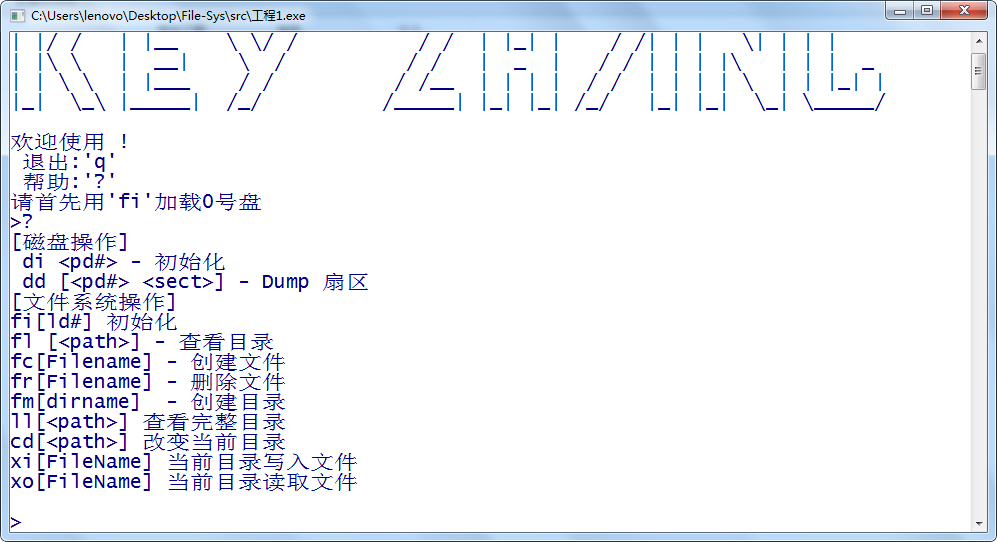
\includegraphics[width=\textwidth]{help.jpg}
  \caption{帮助界面}
  \label{}
  \end{figure}
  \begin{figure}
  \centering
  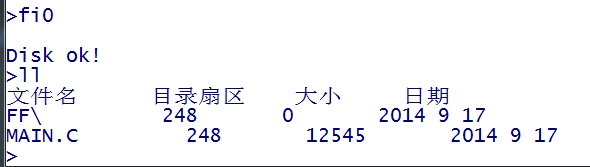
\includegraphics[width=\textwidth]{ll.jpg}
  \caption{读取目录}
  \label{}
  \end{figure}
  \begin{figure}
  \centering
  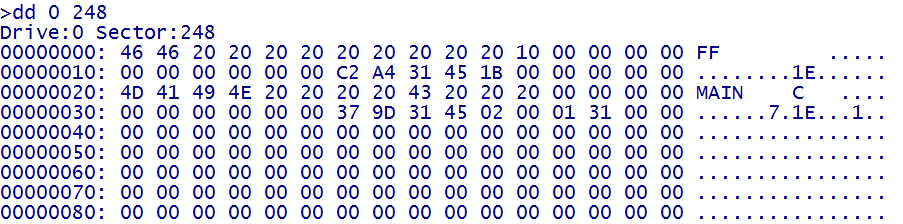
\includegraphics[width=\textwidth]{dd.jpg}
  \caption{Dump}
  \label{}
  \end{figure}
  \begin{figure}
  \centering
  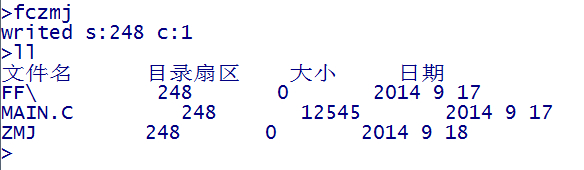
\includegraphics[width=\textwidth]{fc.jpg}
  \caption{创建文件}
  \label{}
  \end{figure}
  \begin{figure}
  \centering
  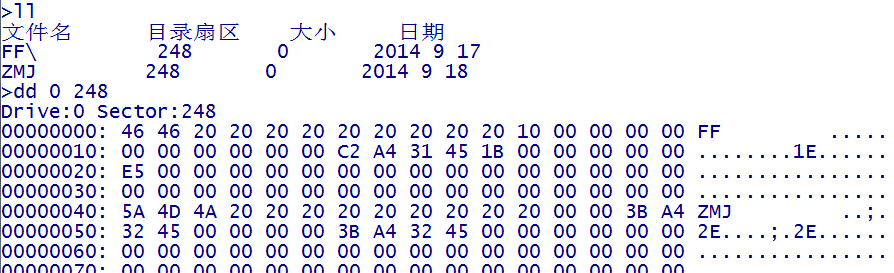
\includegraphics[width=\textwidth]{fr2.jpg}
  \caption{执行 frmain.c 后}
  \label{}
  \end{figure}
\pagebreak
\section{附加功能}
\begin{description}
  \item[xi $<$Filename$>$] 从外部写入磁盘
  \item[xo $<$Filename$>$] 从磁盘读取到data文件夹下
  \item[xp $<$Filename$>$] 用画图打开
  \item[xt $<$Filename$>$] 用记事本打开\footnote{此功能调用系统仅供试用}
\end{description}

\chapter{代码与算法}
\paragraph{} 注意:本程序主要代码额外存放于fun.c中,只用于展示,并未参与编译。
\section{程序结构简介}
\paragraph{} 本程序主要分为三层,分别为底层驱动位于diskio.c,文件系统层ff.c,上层应用main.c,并分别对应有头文件。
  \begin{figure}
  \centering
  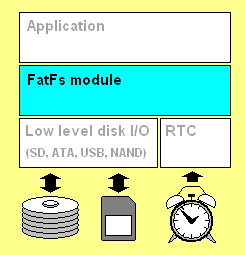
\includegraphics[width=0.3\textwidth]{layers.jpg}
  \caption{程序结构}
  \label{}
  \end{figure}

\section{底层驱动}
\pagebreak
\begin{lstlisting}[language={[ANSI]C}]
  DRESULT disk_read (
    BYTE pdrv,
    BYTE *buff,  '缓存'
    DWORD sector,'扇区编号'
    UINT count   '读写数')
  {
    DRESULT res;
    char a[255];
    sprintf(a,"%d.img",pdrv);
    fp=fopen(a,"rb+");
    fseek(fp,sector*512,0);
    fread(buff, count,512,fp);
    fclose(fp);
    return 0;
  }

DRESULT disk_write (
  BYTE pdrv,
  const BYTE *buff,
  DWORD sector,
  UINT count
)
{
  DRESULT res;
  char a[255];
  sprintf(a,"%d.img",pdrv);
  fp=fopen(a,"rb+");
  fseek(fp,sector*512,0);
  fwrite(buff, 512,count,fp);
  fflush(fp);
  fclose(fp);
  printf("writed s:%d c:%d\n",sector,count);
  return 0;
}
'获取时间'
DWORD get_fattime(){
  int year,month,date,hour,minute,second;
  struct tm *local;
  time_t t;
  t=time(NULL);
  local=localtime(&t);

  year = local->tm_year + 1900;
  month = local->tm_mon+1;
  date = local->tm_mday;
  hour = local->tm_hour;
  minute = local->tm_min;
  second = local->tm_sec;

  return    ((DWORD)(year - 1980) << 25)
      | ((DWORD)month << 21)
      | ((DWORD)date << 16)
      | (WORD)(hour << 11)
      | (WORD)(minute << 5)
      | (WORD)(second >> 1);
}

\end{lstlisting}

\section{文件系统简介}
\subsection{头文件}
\paragraph{} 文件系统各个函数之间的数据传递依靠以下结构和常量:
\begin{lstlisting}[language={[ANSI]C}]

/* '文件系统结构' */
typedef struct {
  BYTE  fs_type;    /*  '分区类型' */
  BYTE  drv;      /* '驱动器编号(012文件名)'*/
  BYTE  csize;      /* '单簇扇区数 1' */
  BYTE  n_fats;     /* 'fat数 (1 or 2)' */
  BYTE  wflag;      /* '是否有缓存等待写入'*/
  BYTE  fsi_flag;   /*  '是否分区表 '*/
  WORD  id;       /* '读写标识'*/
  WORD  n_rootdir;    /* '根目录文件数'*/
  DWORD last_clust;   /*  '最后分配簇'*/
  DWORD free_clust;   /* '空闲簇'*/
  DWORD n_fatent;   /* 'fat记录类型数(簇数+空闲+损坏)'*/
  DWORD fsize;      /*  'fat记录的扇区数'*/
  DWORD volbase;    /* '卷开始扇区' */
  DWORD fatbase;    /* 'FAT记录开始'*/
  DWORD dirbase;    /*  '根目录起始扇区'*/
  DWORD database;   /* '数据起始'*/
  DWORD winsect;    /*'当前缓存的扇区位置'*/
  BYTE  win[512]; /*  '缓存'*/
} FATFS;



/* '文件存储结构'*/

typedef struct {
  FATFS*  fs;       /* '文件系统指针(指向上面的结构)'*/
  DWORD fsize;      /* '大小'*/
  DWORD sclust;     /* '起始簇'*/
  //DWORD clust;      /* '当前指针指向的簇' */
  DWORD dsect;      /* '缓存中扇区'*/
  DWORD dir_sect;   /*  '目录记录所在扇区'*/
  BYTE* dir_ptr;    /* '指向目录记录的指针'*/
  BYTE  buf[512]; /*  '文件读写缓存'*/
} FIL;



/*  目录结构*/

typedef struct {
  FATFS*  fs;       /*  */
  WORD  index;      /*  '当前读写文件索引号'*/
  DWORD sclust;     /* '起始簇(根目录标识为0)'*/
  DWORD clust;      /*  '当前簇'*/
  DWORD sect;     /*  */
  BYTE* dir;      /*  '缓存中的目录记录指针'*/
  BYTE* fn;       /* '缓存中的本目录文件名指针'*/
} DIR;



/* '文件信息结构(从目录记录读取)'*/

typedef struct {
  DWORD fsize;      /*  '大小'*/
  WORD  fdate;      /*  '编辑日期'*/
  WORD  ftime;      /* '时间'*/
  BYTE  fattrib;    /*  '属性'*/
  TCHAR fname[13];    /* '文件名'*/
} FILINFO;
//'小头转换'
#define LD_WORD(ptr)
  (WORD)(((WORD)*((BYTE*)(ptr)+1)<<8)|
  (WORD)*(BYTE*)(ptr))
#define LD_DWORD(ptr)
  (DWORD)(((DWORD)*((BYTE*)(ptr)+3)<<24)|
  ((DWORD)*((BYTE*)(ptr)+2)<<16)|
  ((WORD)*((BYTE*)(ptr)+1)<<8)|*(BYTE*)(ptr))
#define ST_WORD(ptr,val)
  *(BYTE*)(ptr)=(BYTE)(val);
  *((BYTE*)(ptr)+1)=(BYTE)((WORD)(val)>>8)
#define ST_DWORD(ptr,val)
  *(BYTE*)(ptr)=(BYTE)(val);
  *((BYTE*)(ptr)+1)=(BYTE)((WORD)(val)>>8);
  *((BYTE*)(ptr)+2)=(BYTE)((DWORD)(val)>>16);
  *((BYTE*)(ptr)+3)=(BYTE)((DWORD)(val)>>24)


/*  '文件属性'*/

#define AM_RDO  0x01  /* '只读' */
#define AM_HID  0x02  /* '隐藏' */
#define AM_SYS  0x04  /* System */
#define AM_VOL  0x08  /* Volume label */
#define AM_LFN  0x0F  /* LFN entry */
#define AM_DIR  0x10  /* Directory */
#define AM_ARC  0x20  /* Archive */
#define AM_MASK 0x3F  /* Mask of defined bits */
\end{lstlisting}
\subsection{缓存机制}
\paragraph{} 通过缓存1个扇区做到各个函数之间能够直接调用缓存而不是重新读盘:
\begin{lstlisting}[language={[ANSI]C}]
/*'缓存扇区 至内存'*/
static
FRESULT move_window (
  FATFS* fs,    /*  */
  DWORD sector  /*  '缓存扇区编号'*/
)
{
  if (sector != fs->winsect) {  /*  '改变当前读写窗口'*/
    if (sync_window(fs) != FR_OK)
      return FR_DISK_ERR;
    if (disk_read(fs->drv, fs->win, sector, 1))
      return FR_DISK_ERR;
    fs->winsect = sector;
  }

  return FR_OK;
}
/*'确认缓存写入完成(同步读写窗口)'*/
static
FRESULT sync_window (
  FATFS* fs   /* File system object */
)
{
  DWORD wsect;
  UINT nf;


  if (fs->wflag) {  /*  '检查是否缓存'*/
    wsect = fs->winsect;  /* '当前缓存的扇区地址'*/
    if (disk_write(fs->drv, fs->win, wsect, 1))
      return FR_DISK_ERR;
    fs->wflag = 0;
    if (wsect - fs->fatbase < fs->fsize) {
      /*'判断是否在fat区'*/
      for (nf = fs->n_fats; nf >= 2; nf--) {
        /* '写入到其他fat拷贝'*/
        wsect += fs->fsize;
        disk_write(fs->drv, fs->win, wsect, 1);
      }
    }
  }
  return FR_OK;
}
\end{lstlisting}
\subsection{FAT表操作}
\paragraph{} 在操作FAT表的时候经常需要计算簇和扇区对应关系以及FAT记录所在位置,本块函数主要解决FAT表读写和链的操作\footnote{包括新建,删除以及延长}

\begin{lstlisting}[language={[ANSI]C}]
/*'从簇得扇区'*/
DWORD clust2sect (
  FATFS* fs,
  DWORD clst
)
{
  clst -= 2;
  if (clst >= (fs->n_fatent - 2)) return 0;
  return clst * fs->csize + fs->database;
}
/*'簇读取fat中入口并返回默认为fat16'*/
DWORD get_fat (
  FATFS* fs,
  DWORD clst
)
{
  UINT wc, bc;
  BYTE *p;


  if (clst < 2 || clst >= fs->n_fatent)
    return 1;
    move_window(fs,fs->fatbase+(clst/(SS(fs)/2)));
    /*'16位的fat所以除2'*/
    p = &fs->win[clst * 2 % SS(fs)];
    return LD_WORD(p);
  return 0xFFFFFFFF;  /* '错误' */
}


/*'簇写入fat入口'*/


FRESULT put_fat (
  FATFS* fs,
  DWORD clst,
  DWORD val
)
{
  UINT bc;
  BYTE *p;
  FRESULT res;


  if (clst < 2 || clst >= fs->n_fatent) {
    res = FR_INT_ERR;
  } else {
      res = move_window(fs,fs->fatbase+(clst/(SS(fs)/2)));
      res != FR_OK;
      p = &fs->win[clst * 2 % SS(fs)];
      ST_WORD(p, (WORD)val);/*'16位小头存储'*/
    fs->wflag = 1;/*'标记缓存未写入状态'*/
    sync_window(fs);
  }
  return res;
}

/*'创建链表'*/
static
DWORD create_chain (
  FATFS* fs,
  DWORD clst
)
{
  DWORD cs, ncl, scl;
  FRESULT res;


  if (clst == 0) {    /* '创建新链' */
    scl = fs->last_clust;
     /* '从最前的从未分配空簇开始' */
    if (!scl || scl >= fs->n_fatent) scl = 1;
    /*'所有簇都已经分配过'*/
  }
  else {          /* '连接' */
    cs = get_fat(fs, clst);
    /*  *'检查开始簇是否空'*/
    if (cs < fs->n_fatent) return cs;
    /* '已经占用'*/
    scl = clst;
  }

  ncl = scl;
  /*循环直到找到下一个空簇*/
  for (;;) {
    ncl++;
    if (ncl >= fs->n_fatent) {    /* '回到开头' */
      ncl = 2;
      if (ncl > scl) return 0;
    }
    cs = get_fat(fs, ncl);
    if (cs == 0) break;       /*  '找到空簇'*/
    if (ncl == scl) return 0;   /* '没了' */
  }

  res = put_fat(fs, ncl, 0x0FFFFFFF); /* '标记为文件结束' */
  if (res == FR_OK && clst != 0) {
    res = put_fat(fs, clst, ncl); /* '与上一个连接' */
  }
  if (res == FR_OK) {
    fs->last_clust = ncl;     /* '更新文件系统' */
    if (fs->free_clust != 0xFFFFFFFF) {
      fs->free_clust--;
      fs->fsi_flag |= 1;
    }
  } else {
    ncl = (res == FR_DISK_ERR) ? 0xFFFFFFFF : 1;
  }

  return ncl;   /* '返回新簇'*/
}
/*'清除链表'*/
static
FRESULT remove_chain (
  FATFS* fs,
  DWORD clst
)
{
  FRESULT res;
  DWORD nxt;


  if (clst < 2 || clst >= fs->n_fatent) {
    res = FR_INT_ERR;

  } else {
    res = FR_OK;
    while (clst < fs->n_fatent) {
      /* '判断是否超出范围'*/
      nxt = get_fat(fs, clst);
      res = put_fat(fs, clst, 0);
      /*' 标记当前簇为空' */
      if (res != FR_OK) break;
      if (fs->free_clust != 0xFFFFFFFF) {
        /* '更新文件系统 增加空扇区计数'*/
        fs->free_clust++;
        fs->fsi_flag |= 1;
        /*'标记等待写入'*/
      }

      clst = nxt;
    }
  }

  return res;
}
\end{lstlisting}
\subsection{目录操作}
\paragraph{}主要是目录记录的读取写入,以及我自己写的使用方案
\begin{lstlisting}[language={[ANSI]C}]

//'获取目录信息'
FRESULT f_opendir (
  DIR* dp,
  const TCHAR* path
)
{
  FRESULT res;
  FATFS* fs;
  DEF_NAMEBUF;


  if (!dp) return FR_INVALID_OBJECT;
  if (res == FR_OK) {
    dp->fs = fs;
    if (res == FR_OK) {
      if (dp->dir) {
        if (dp->dir[DIR_Attr] & AM_DIR)
          dp->sclust = ld_clust(fs, dp->dir);
        else              /* '目标是文件' */
          res = FR_NO_PATH;
      }
      if (res == FR_OK) {
        dp->id = fs->id;
        res = dir_sdi(dp, 0);

      }
    }

  }
}

//'获取文件信息'
static
void get_fileinfo (
  DIR* dp,
  FILINFO* fno
)
{
  UINT i;
  TCHAR *p, c;


  p = fno->fname;
  if (dp->sect) {   /*' 获取名称'*/
    BYTE *dir = dp->dir;/*'目录索引目标名称'*/
    i = 0;
    while (i < 11) {    /*  '文件名和扩展名'*/
      c = (TCHAR)dir[i++];
      if (c == ' ') continue;     /* '跳过空格' */
      if (i == 9) *p++ = '.';     /*  '扩展名'*/
      *p++ = c;
    }
    fno->fattrib = dir[DIR_Attr];
    /*  '读取属性'*/
    fno->fsize = LD_DWORD(dir+DIR_FileSize);
    /*  '大小'*/
    fno->fdate = LD_WORD(dir+DIR_WrtDate);
    /* Date */
    fno->ftime = LD_WORD(dir+DIR_WrtTime);
    /* Time */
  }
  *p = 0;   /* Terminate SFN string by a \0 '文件名结束'*/
}

'使用方案:针对区分目录的文件读写策略'
    if(dp->sclust)
        disk_read(0,buff,clust2sect(dp->fs,dp->sclust),1);
    else
        disk_read(0,buff,dp->fs->dirbase,1);
    '先判断是否是根目录,设定缓存读取扇区'
    if(dp->sclust)
      disk_write(0,buff,clust2sect(dp->fs,dp->sclust),1);
    else
      disk_write(0,buff,dp->fs->dirbase,1);
    '缓存写入对应的数据之后,写入对应扇区,
    从而避免对其它读写缓存的影响'
\end{lstlisting}
\section{交互界面简介}
\paragraph{}交互界面采用控制台模式,通过switch-case得到命令之后继续读取得到参数从而既避免
了二次读取参数又保证了后续的可升级性。下面贴出参数处理的重要函数:
\begin{lstlisting}[language={[ANSI]C}]
//'用于分离参数中的数值,并且可以识别不同进位制'
int xatoi (
    TCHAR **str,
    long *res
)
{
    unsigned long val;
    unsigned char r, s = 0;
    TCHAR c;


    *res = 0;
    while ((c = **str) == ' ') (*str)++;
    //'跳过空格'

    if (c == '-') {     /* 负数 */
        s = 1;
        c = *(++(*str));
    }

    if (c == '0') {
        c = *(++(*str));
        switch (c) {
        case 'x':
            r = 16; c = *(++(*str));
            break;
        case 'b':
            r = 2; c = *(++(*str));
            break;
        default:
            if (c <= ' ') return 1;
            if (c < '0' || c > '9') return 0;
            r = 8;
        }
    } else {
        if (c < '0' || c > '9') return 0;
        r = 10;
    }

    val = 0;
    while (c > ' ') {
        if (c >= 'a') c -= 0x20;
        c -= '0';
        if (c >= 17) {
            c -= 7;
            if (c <= 9) return 0;
        }
        if (c >= r) return 0;
        val = val * r + c;
        c = *(++(*str));
    }
    if (s) val = 0 - val;

    *res = val;
    return 1;
}
\*------------------'系统调用'-----------------*\
    char c[126]="mspaint .\\data\\";
    char d[126]="mspaint .\\data\\";
    char t[126]="notepad .\\data\\";
    char tt[126]="notepad .\\data\\";
    case 'p': xcopy(&dir,ptr); strcpy(c,d);
    strcat(c,ptr);
    system(c);
    break;
    case 't': xcopy(&dir,ptr); strcpy(t,tt);
    strcat(t,ptr);
    system(t);
    break;
    \*'最后突发奇想利用系统调用外部命令查看从磁盘里读取的文件
    并且在应用开始打开磁盘管理'*\
\end{lstlisting}
\chapter{总结}
\section{感谢}
\paragraph{}
在这次作业过程中我参考了许多开源的文件系统,在很大程度上帮助了我对于FAT文件系统的理解,
并且在作品中也多少用到了他们的成果,在最后要感谢这些无私贡献的码农们。
感谢:
\begin{itemize}
  \item  FatFs - FAT file system module  R0.10b  (C)ChaN, 2014
  \item  cnFat Tony Yang,2007
\end{itemize}
\section{版权}
\paragraph{} 在这份代码中包含了部分基于FatFs的代码
\paragraph{} FatFs module is a generic FAT file system module for small embedded systems.
This is a free software that opened for education, research and commercial
developments under license policy of following terms.
\paragraph{}
Copyright (C) 2014, ChaN, all right reserved.
\paragraph{}
The FatFs module is a free software and there is NO WARRANTY.
No restriction on use. You can use, modify and redistribute it for
personal, non-profit or commercial products UNDER YOUR RESPONSIBILITY.
Redistributions of source code must retain the above copyright notice.
\paragraph{}
本程序开源代码公开于 https://github.com/zmj1316/File-Sys
\paragraph{}
更多关于FAT文件系统的文档参阅http://msdn.microsoft.com/en-us/windows/hardware/gg463080.aspx
\end{CJK}
\end{document}
